\documentclass{IEEEtran}
\usepackage[T1]{fontenc}
\usepackage[utf8]{inputenc}
\usepackage[brazil]{babel}
\usepackage{graphicx}
\usepackage{amsmath}
\usepackage{amssymb}
\usepackage{cite}
\usepackage{booktabs}
\usepackage{hyperref}
\usepackage{url}
\usepackage{natbib}
\usepackage{enumitem}
\usepackage{array}
\usepackage{multirow}
\usepackage{xcolor}
\usepackage[table]{xcolor}
\usepackage{array}

\markboth{}{PLN -- UFSCar 2026: Projeto de Processamento de Linguagem Natural}

\title{Sentimento como Relevância: Recomendação de Produtos em E-commerce Brasileiro}

\author{%
  Cilene Renata Real$^{1}$,
  Jayme Sakae dos Reis Furuyama$^{1}$,
  Wesley Nogueira Galvão 3$^{1}$,
  $^{1}$Programa de Pós-Graduação em Ciência da Computação (PPGCC),
  Universidade Federal de São Carlos (UFSCar), São Carlos, SP, Brasil\\
  \texttt{\{real.cilene, jaymefuryama\}@gmail.com}\\
  \texttt{wesleygalvao@estudante.ufscar.br}
}

\begin{document}
\maketitle

% =========================================================
\begin{abstract}
A análise de sentimentos em avaliações de produtos é uma das tarefas mais estudadas em Processamento de Linguagem Natural (PLN), com forte aplicabilidade em plataformas de e-commerce. Este trabalho propõe um sistema integrado de duas etapas: (i)~um classificador de polaridade de sentimento (positivo/negativo) a ser treinado sobre avaliações em português brasileiro do corpus B2W-Reviews01, comparando representações baseadas em TF-IDF e \textit{embeddings} contextuais do BERTimbau; e (ii)~um motor de recomendação de produtos que recuperará itens semanticamente similares pelo título, re-ranqueando os resultados por um \textit{score} de positividade derivado do modelo com melhor desempenho. Os classificadores serão avaliados com precisão, revocação, F1-macro e AUC-ROC, e o módulo de recomendação com NDCG@k e Precision@k, complementados por avaliação qualitativa conduzida pelos integrantes do grupo. Espera-se que a combinação de representações densas com análise de sentimento agregue valor significativo à qualidade das recomendações em domínios ruidosos de texto gerado por usuário.
\end{abstract}

% =========================================================
\section{Introdução}
\label{sec:intro}

Plataformas de comércio eletrônico acumulam diariamente volumes massivos de avaliações escritas por consumidores. Essas avaliações constituem uma fonte rica de opinião sobre produtos, entrega e experiência de compra, porém permanecem majoritariamente subutilizadas nos sistemas de recomendação tradicionais, que tendem a depender exclusivamente de dados de interação (cliques, compras e notas numéricas) \cite{ahmed2025sentimentaware}.

Análise de sentimentos (AS) é a tarefa de PLN que visa inferir automaticamente a polaridade afetiva de um texto partir de seu conteúdo \cite{alzahrani2022intelligent}. O seu objetivo é estudar e extrair opiniões, avaliações, atitudes, apreciações e emoções direcionadas a entidades como produtos, serviços, indivíduos, tópicos ou eventos \cite{BPLN_livro_4ed:2026}. A análise pode ser conduzida em três níveis de granularidade: no nível do documento (avaliando a polaridade geral do texto), no nível da sentença, ou no nível do aspecto

Quando aplicada a avaliações de produtos, ela permite mapear opiniões para um sinal de qualidade que complementa a nota numérica fornecida pelo consumidor. O corpus B2W-Reviews01 \cite{real2019b2w}, formado por mais de 130 mil avaliações da Americanas.com em português brasileiro, é um recurso público representativo desse domínio, com anotações de nota (1--5 estrelas), recomendação binária e metadados demográficos dos avaliadores.

Dois desafios fundamentais motivam este projeto. O primeiro é a representação adequada do texto em português para tarefas de classificação: abordagens baseadas em vetorização esparsa oferecem uma linha de base eficiente e interpretável \cite{BPLN_livro_4ed:2026}, enquanto modelos de vetorização densa capturam dependências semânticas e contextuais que as superam em diversas tarefas \cite{jm3}. O segundo desafio é a integração do sinal de sentimento em um motor de recomendação: recuperar produtos similares pelo título por meio de busca vetorial e re-ranquear os resultados pelo índice de positividade das avaliações classifica melhor os itens que os consumidores efetivamente recomendam.

Desta forma, o presente projeto propõe um \textit{pipeline} completo que: (a) realiza análise exploratória e pré-processamento do corpus B2W-Reviews01; (b) compara dois paradigmas de representação textual para classificação de sentimento binária; (c) constrói um banco vetorial dos títulos de produtos; e (d) entrega recomendações re-ranqueadas pelo sentimento. O sistema final é avaliado tanto quantitativamente quanto por análise qualitativa conduzida pelos integrantes do grupo.

O restante do relatório está organizado da seguinte forma: a Seção~\ref{sec:related} apresenta os trabalhos relacionados; a Seção~\ref{sec:methodology} descreve a metodologia detalhada; e a Seção~\ref{sec:conclusion} traz as considerações finais e os próximos passos.

% =========================================================
\section{Trabalhos Relacionados}
\label{sec:related}

\subsection{Análise de Sentimentos em Avaliações de E-commerce}

% A análise de sentimentos em avaliações de produtos é uma área amplamente estudada. \citeauthor{alzahrani2022intelligent}~\cite{alzahrani2022intelligent} propuseram um sistema baseado em aprendizado profundo combinando CNN, LSTM e BERT para classificar avaliações de e-commerce em múltiplas polaridades, obtendo acurácia superior a 94\% em conjuntos de dados em inglês. Os autores destacam que avaliações são ruidosas -- com erros tipográficos, gírias e linguagem informal -- e que o pré-processamento adequado é fundamental para o desempenho dos modelos.
%  Ajeitando a citação
A análise de sentimentos em avaliações de produtos é uma área amplamente estudada. Alzahrani \textit{et al.}~\cite{alzahrani2022intelligent} propuseram um sistema baseado em aprendizado profundo combinando CNN, LSTM e BERT para classificar avaliações de e-commerce em múltiplas polaridades, obtendo acurácia superior a 94\% em conjuntos de dados em inglês. Os autores destacam que avaliações são ruidosas, com erros tipográficos, gírias e linguagem informal, e que o pré-processamento adequado é fundamental para o desempenho dos modelos.

% Para o português brasileiro, a situação é mais desafiadora pela escassez de recursos anotados. \citeauthor{souza2022bert}~\cite{souza2022bert} realizaram um estudo comparativo sistemático entre TF-IDF com Regressão Logística (linha de base), embeddings do BERTimbau (pré-treinado sem ajuste fino) e BERTimbau com \textit{fine-tuning} em datasets de sentimento em português. Os autores demonstraram que o BERTimbau com \textit{fine-tuning} supera consistentemente a linha de base TF-IDF, atingindo AUC-ROC superior a 0.95 em múltiplos benchmarks, e que a versão \textit{large} do modelo apresenta ganhos marginais em relação à versão \textit{base}.

%  Ajeitando a citação
Para o português brasileiro, a situação é mais desafiadora pela escassez de recursos anotados. Sousa e Filho\cite{souza2022bert} realizaram um estudo comparativo sistemático entre TF-IDF com Regressão Logística (linha de base), embeddings do BERTimbau (pré-treinado sem ajuste fino) e BERTimbau com \textit{fine-tuning} em datasets de sentimento em português. Os autores demonstraram que o BERTimbau com \textit{fine-tuning} supera consistentemente a linha de base TF-IDF, atingindo AUC-ROC superior a 0.95 em múltiplos benchmarks, e que a versão \textit{large} do modelo apresenta ganhos marginais em relação à versão \textit{base}.


\subsection{Modelos de Linguagem Pré-treinados: BERT e BERTimbau}

O BERT (\textit{Bidirectional Encoder Representations from Transformers}) \cite{devlin2019bert} revolucionou o PLN ao propor o pré-treinamento bidirecional profundo sobre grandes corpora, seguido de \textit{fine-tuning} supervisionado para tarefas específicas. Diferente de modelos anteriores, o BERT condiciona simultaneamente os contextos esquerdo e direito em todas as suas camadas de atenção, produzindo representações contextuais ricas.

O BERTimbau \cite{souza2020bertimbau} é a adaptação do BERT para o português brasileiro, pré-treinado no corpus BrWaC (\textit{Brazilian Web as Corpus}) com aproximadamente 2,7 bilhões de palavras. O modelo está disponível nas versões \textit{base} (110M parâmetros) e \textit{large} (335M parâmetros) e estabeleceu novos estados da arte em reconhecimento de entidades nomeadas, similaridade textual e implicação textual em português.

\subsection{TF-IDF como Representação para Classificação de Texto}

A ponderação TF-IDF (\textit{Term Frequency--Inverse Document Frequency}) \cite{manning2008introduction} é uma das representações esparsas mais utilizadas em tarefas de classificação de texto. Combinada com classificadores lineares como a Regressão Logística, essa abordagem serve como linha de base interpretável e de baixo custo computacional. Por não capturar dependências contextuais, o TF-IDF com Regressão Logística pode, em certos cenários, apresentar desempenho competitivo frente a modelos mais complexos, especialmente em domínios com vocabulário especializado e textos curtos \cite{souza2022bert}.

\subsection{Recomendação de Produtos Orientada por Sentimento}
% Ajeitando citação
% A integração de análise de sentimentos em sistemas de recomendação tem crescido significativamente. \citeauthor{vaishnavi2023sentiment}~\cite{vaishnavi2023sentiment} propuseram um sistema que combina classificação de sentimento das avaliações com XGBoost e CatBoost e usa a saída para construir matrizes de similaridade item-item baseadas em similaridade de cosseno, reportando melhorias no RMSE frente a sistemas baseados apenas em notas numéricas. 

A integração de análise de sentimentos em sistemas de recomendação tem crescido significativamente. Vaishnavi e Kalpana~\cite{vaishnavi2023sentiment} propuseram um sistema que combina e classifica o sentimento das avaliações com XGBoost e CatBoost e usa a saída para construir matrizes de similaridade item-item baseadas em similaridade de cosseno, reportando melhorias no RMSE frente a sistemas baseados apenas em notas numéricas.


Uma revisão abrangente recente \cite{ahmed2025sentimentaware} categoriza os sistemas de recomendação orientados por sentimento em quatro grandes abordagens: (i) classificadores de aprendizado profundo que combinam embeddings de sentimento com interações usuário-item; (ii) métodos baseados em Transformers para extração de features; (iii) redes neurais em grafos que propagam sinais de sentimento; e (iv) recomendadores conversacionais que se adaptam em tempo real ao \textit{feedback} do usuário. O trabalho de Darraz \textit{et al.}~\cite{sharma2025enhancing} demonstrou que incorporar sentimento via BERT em filtragem colaborativa reduz o RMSE para 1,2478 em benchmarks do Yelp, reforçando a relevância da abordagem proposta neste projeto.

% Ajeitando citação
% Uma revisão abrangente recente \cite{ahmed2025sentimentaware} categoriza os sistemas de recomendação orientados por sentimento em quatro grandes abordagens: (i) classificadores de aprendizado profundo que combinam embeddings de sentimento com interações usuário-item; (ii) métodos baseados em Transformers para extração de features nuançadas; (iii) redes neurais em grafos que propagam sinais de sentimento; e (iv) recomendadores conversacionais que se adaptam em tempo real ao \textit{feedback} do usuário. O trabalho de \citeauthor{sharma2025enhancing}~\cite{sharma2025enhancing} demonstrou que incorporar sentimento via BERT em filtragem colaborativa reduz o RMSE para 1,2478 em benchmarks do Yelp, reforçando a relevância da abordagem proposta neste projeto.

% =========================================================
\section{Metodologia}
\label{sec:methodology}

\subsection{Base de Dados}
\label{subsec:dataset}
O projeto utiliza o corpus B2W-Reviews01 \cite{real2019b2w}, um conjunto de dados aberto de avaliações de produtos coletadas da plataforma Americanas.com entre janeiro e maio de 2018.\footnote{Disponível em \url{https://huggingface.co/datasets/ruanchaves/b2w-reviews01} e \url{https://github.com/americanas-tech/b2w-reviews01}.} A Tabela~\ref{tab:dataset} resume as principais características do corpus.

\begin{table}[htbp]
  \centering
  \caption{Características do corpus B2W-Reviews01}
  \label{tab:dataset}
  \begin{tabular}{ll}
    \toprule
    \textbf{Característica} & \textbf{Valor} \\
    \midrule
    Total de avaliações & 132.373 \\
    Avaliadores únicos & 112.993 \\
    Produtos únicos & 48.001 \\
    Total de tokens & 3.160.781 \\
    Tokens únicos & 148.541 \\
    Mediana de tokens/avaliação & 16 \\
    Período de coleta & Jan--Mai 2018 \\
    Idioma & Português Brasileiro \\
    Produtos com nota negativa (1 e 2) & 27,02\% \\
    Produtos com nota positiva (4 e 5) & 60,66\% \\
    Produtos com nota neutra (3) & 12.33\% \\
    \bottomrule
  \end{tabular}
\end{table}

Cada instância contém: data de submissão, identificador do avaliador, identificador e nome do produto, marca, categorias de primeiro e segundo nível, nota geral (1--5), recomendação binária a um amigo (Sim/Não), título da avaliação, texto completo da avaliação, ano de nascimento, gênero e estado do avaliador.


\subsubsection{Mapeamento de Polaridade}
\label{subsubsec:polarity}

Trabalhos anteriores sobre o corpus B2W-Reviews01 adotam o mapeamento de notas para polaridade binária descartando avaliações com nota 3 por serem consideradas ambíguas \cite{real2019b2w}. Seguindo essa convenção, este trabalho adota o seguinte mapeamento:

\begin{itemize}[noitemsep]
  \item \textbf{Positivo}: notas 4 e 5 estrelas.
  \item \textbf{Negativo}: notas 1 e 2 estrelas.
  \item \textbf{Descartado}: notas 3 estrelas.
\end{itemize}

\subsubsection{Análise Exploratória de Dados}

A etapa de análise exploratória abrange: (i) distribuição de classes pelo mapeamento de polaridade; (ii) distribuição das notas de 1 a 5 estrelas; (iii) análise de dados faltantes nos campos de texto (\texttt{review\_text}, \texttt{review\_title}); (iv) frequência de avaliações por categoria de produto (\texttt{site\_category\_lv1}); (v) comprimento médio dos textos por polaridade; e (vi) nuvem de palavras das revisões mais frequentes por classe. As análises apresentadas nesta seção são parciais e o relatório final contemplará uma exploração mais ampla do corpus.

A Figura~\ref{fig:histograma_ratings} apresenta a distribuição das pontuações no corpus. Observa-se concentração nas notas extremas, com predominância de avaliações positivas sobre as negativas. Após o descarte das avaliações com nota 3, o corpus binário resultante apresenta desbalanceamento moderado entre as classes, que será tratado por meio da aplicação de pesos por classe durante o treinamento, estratégia suportada pelos classificadores investigados, de modo a reduzir o viés do modelo em favor da classe majoritária.



\begin{figure}[htbp]
    \centering
    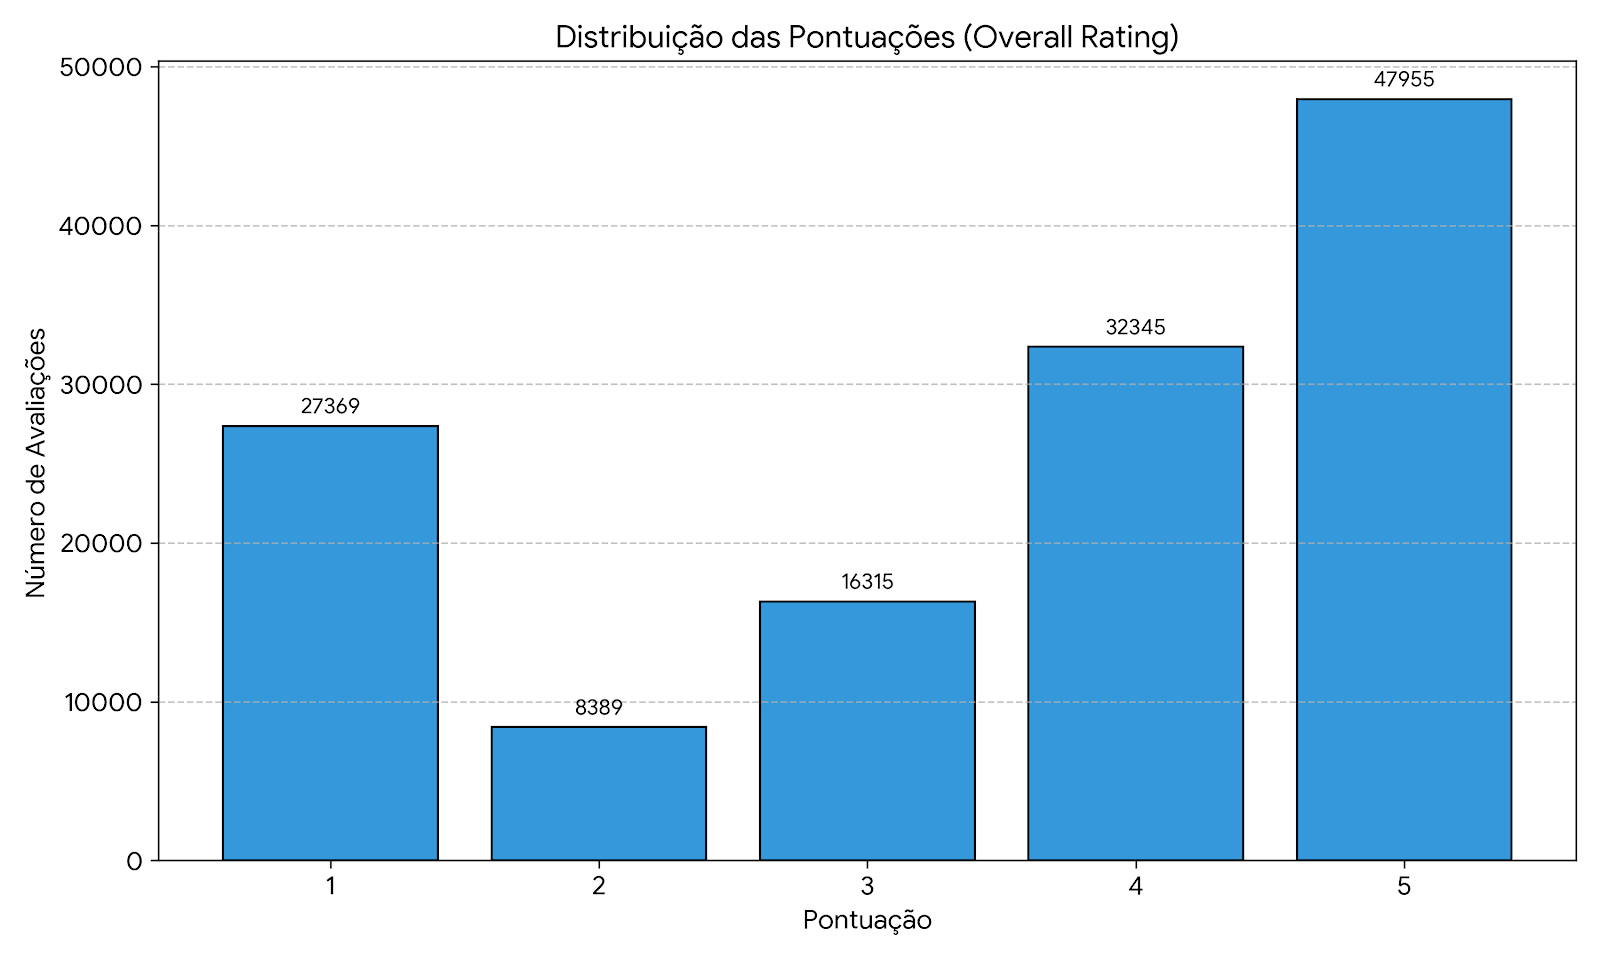
\includegraphics[width=\columnwidth]{figuras/Histograma.png}
    \caption{Distribuição das pontuações (\textit{overall rating}) no corpus B2W-Reviews01. A assimetria entre as notas extremas, com concentração em 1 e 5 estrelas, indica polarização das opiniões dos avaliadores.}
    \label{fig:histograma_ratings}
\end{figure}

Os exemplos da Tabela~\ref{tab:exemplos} ilustram os principais desafios do corpus. No primeiro caso, o texto trata de um problema logístico, devolução de produto avariado, e não de uma opinião sobre o item em si, evidenciando que a polaridade da avaliação pode refletir a experiência de compra e não a qualidade do produto. No segundo, a frustração com a não entrega é reforçada por marcadores de linguagem informal e afetiva (uso excessivo de pontuação e interjeições), fenômeno comum em texto gerado por usuário que desafia modelos baseados em frequência de termos como o TF-IDF. O terceiro caso é o mais crítico para a classificação de sentimentos: o texto é explicitamente negativo, dirigido ao processo de avaliação da plataforma, enquanto a nota e a recomendação são positivas, evidenciando que a polaridade textual nem sempre reflete o sentimento do consumidor sobre o produto~\cite{real2019b2w}.

\begin{table*}[htbp]
    \centering
    \caption{Exemplos de avaliações do corpus B2W-Reviews01}
    \label{tab:exemplos}
    \renewcommand{\arraystretch}{1.4}
    \begin{tabular}{p{0.14\linewidth} p{0.22\linewidth} p{0.38\linewidth} c c}
    \toprule
    \textbf{Produto} & \textbf{Título} & \textbf{Texto} & \textbf{Nota} & \textbf{Recomenda?} \\
    \midrule
    
    Penteadeira JB 7200 com Banqueta Amarelo &
    O produto foi devolvido, devido estar avariado. &
    Gostaria de cancelar esta compra, peço sua gentileza me informar como devo proceder. &
    2 & Não \\
    
    \midrule
    
    Chaleira Elétrica Cadence CEL800 1,7 Litros Inox Prime &
    Eu não recebi o produto????!!!!!!!  &
    Eu não recebi o produto e a americanas sabe disso pois já relatei a reclamação diversas vezes!!! Só vão devolver o dinheiro no procon e isso mesmo????? &
    1 & Não \\
    
    \midrule
    
    Smartphone Multilaser MS80 4G 32GB &
    bom &
    que merda pq n pode so da estrela tem que escrever alguma coisa para avaliar koe americanas muda isso &
    5 & Sim \\
    
    \bottomrule
    \end{tabular}
\end{table*}

A Figura~\ref{fig:palavras_frequentes} sugere um aspecto relevante para o pré-processamento: termos como ``entrega'', ``prazo'' e ``americanas'' figuram entre os mais frequentes, indicando que parte das avaliações pode tratar da experiência de compra e não do produto em si, o que tende a introduzir ruído para a tarefa de classificação de sentimento. A Figura~\ref{fig:categorias_produtos} mostra que o corpus concentra produtos em categorias de eletrônicos, com Celulares e Smartphones representando cerca de 26\% dos produtos únicos. As Figuras~\ref{fig:ranking_categoria} e~\ref{fig:ranking_negativo_categoria}, analisadas em conjunto, indicam que as categorias de maior volume, como Celulares e Smartphones e Eletroportáteis, estão entre as de menor média de rating, ao passo que categorias de nicho como Linha Industrial e Agro, Indústria e Comércio concentram as avaliações mais negativas, apontando para uma distribuição de polaridade heterogênea entre domínios do corpus.

\begin{figure}[htbp]
    \centering
    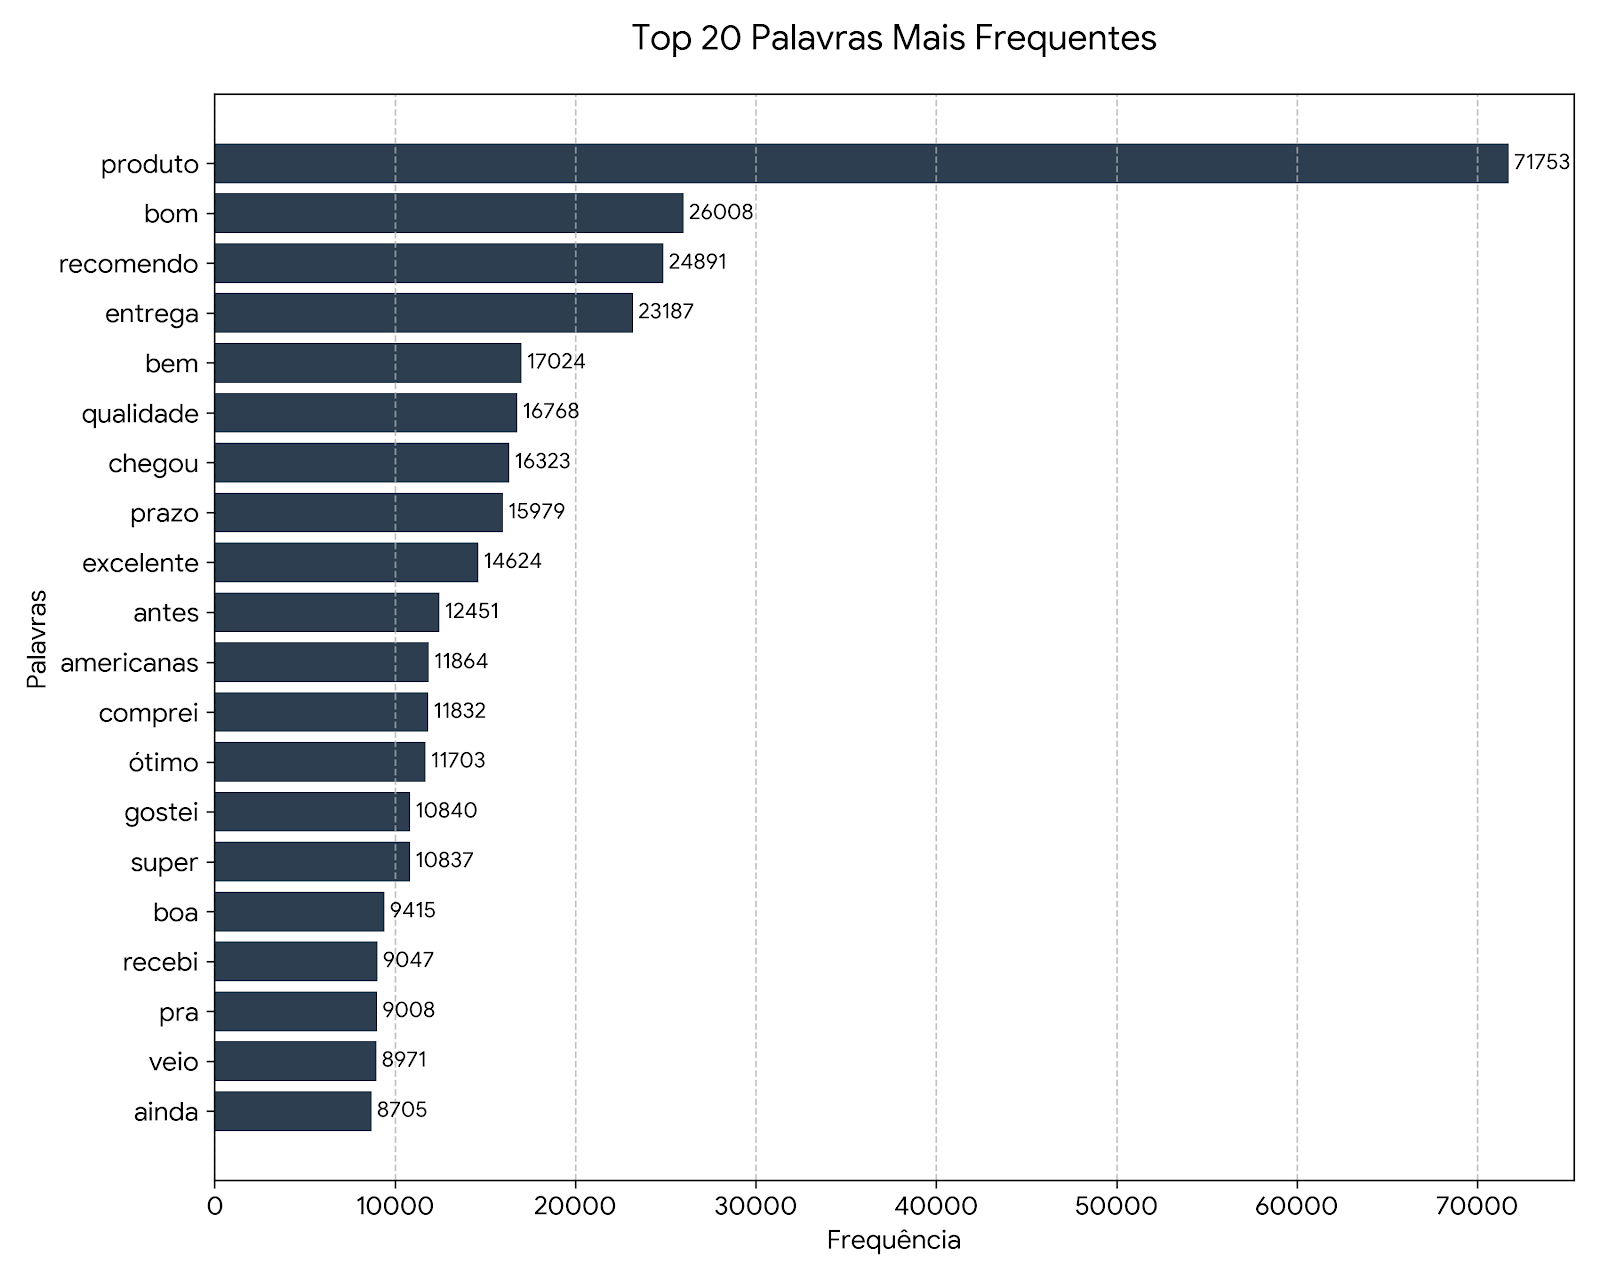
\includegraphics[width=\columnwidth]{figuras/top_20_palavras_frequentes.png}
    \caption{Frequência absoluta das 20 palavras mais recorrentes no corpus B2W-Reviews01 após remoção de \textit{stopwords}. A predominância de termos como ``produto'', ``entrega'' e ``prazo'' evidencia que as avaliações cobrem tanto a qualidade do item quanto a experiência de compra.}
    \label{fig:palavras_frequentes}
\end{figure}

\begin{figure}[htbp]
    \centering
    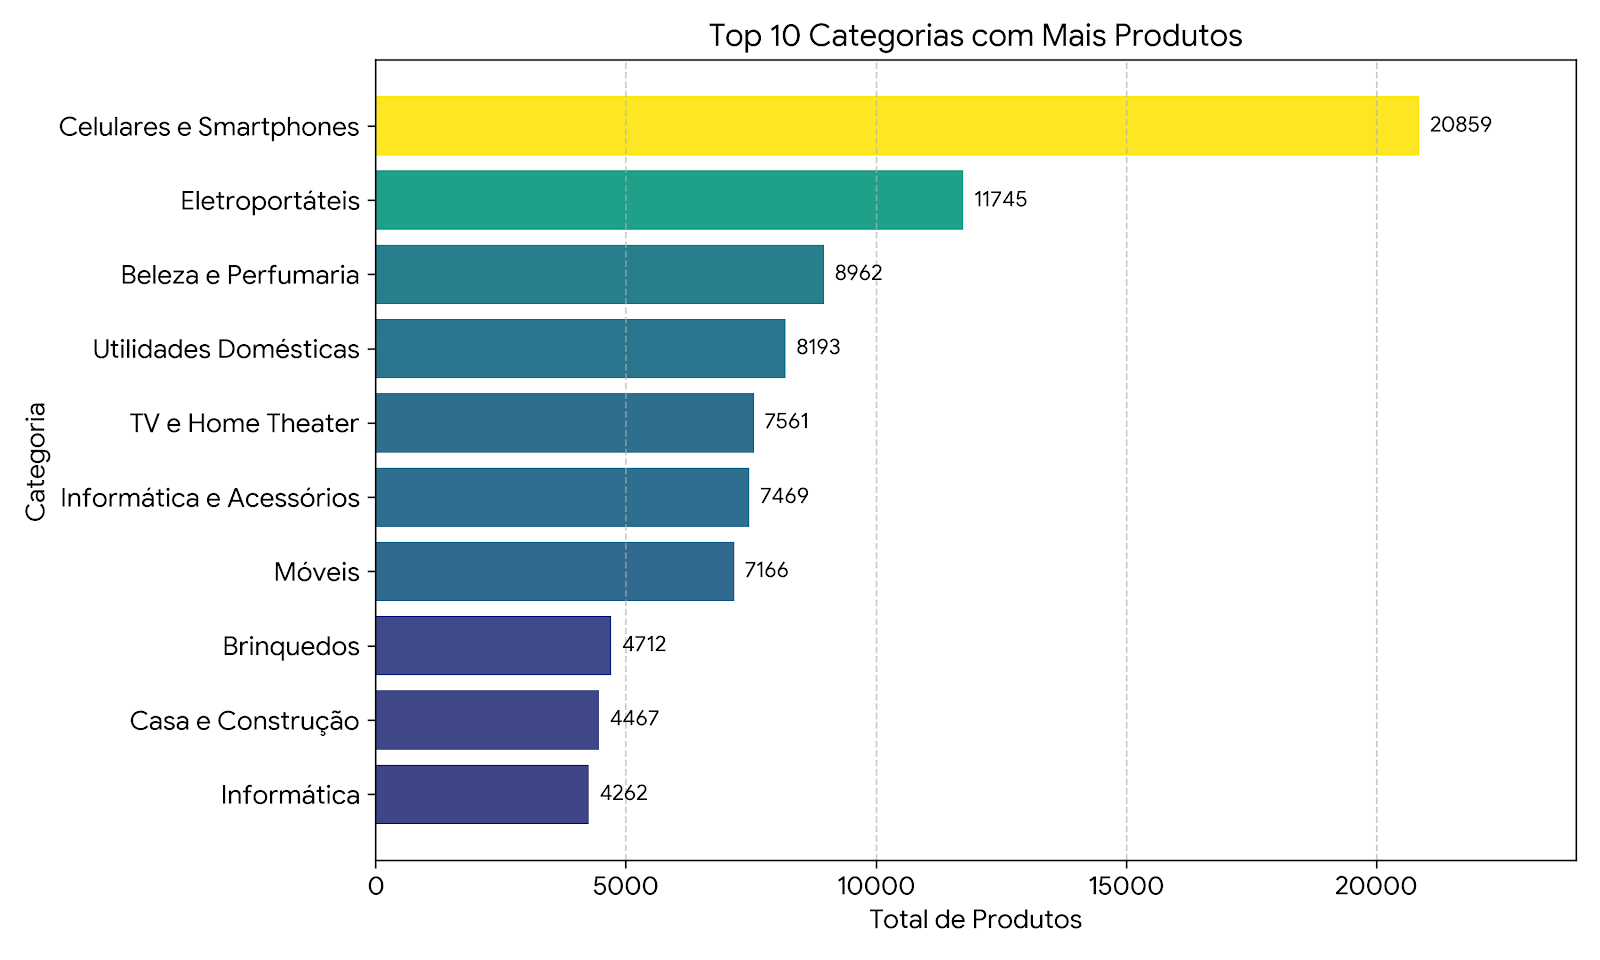
\includegraphics[width=\columnwidth]{figuras/top_categorias_mais_produtos.png}
    \caption{Top 10 categorias de primeiro nível com maior número de produtos únicos no corpus. Celulares e Smartphones concentra quase o dobro de produtos da segunda categoria, indicando forte viés do corpus para eletrônicos de consumo.}
    \label{fig:categorias_produtos}
\end{figure}

\begin{figure}[htbp]
    \centering
    % 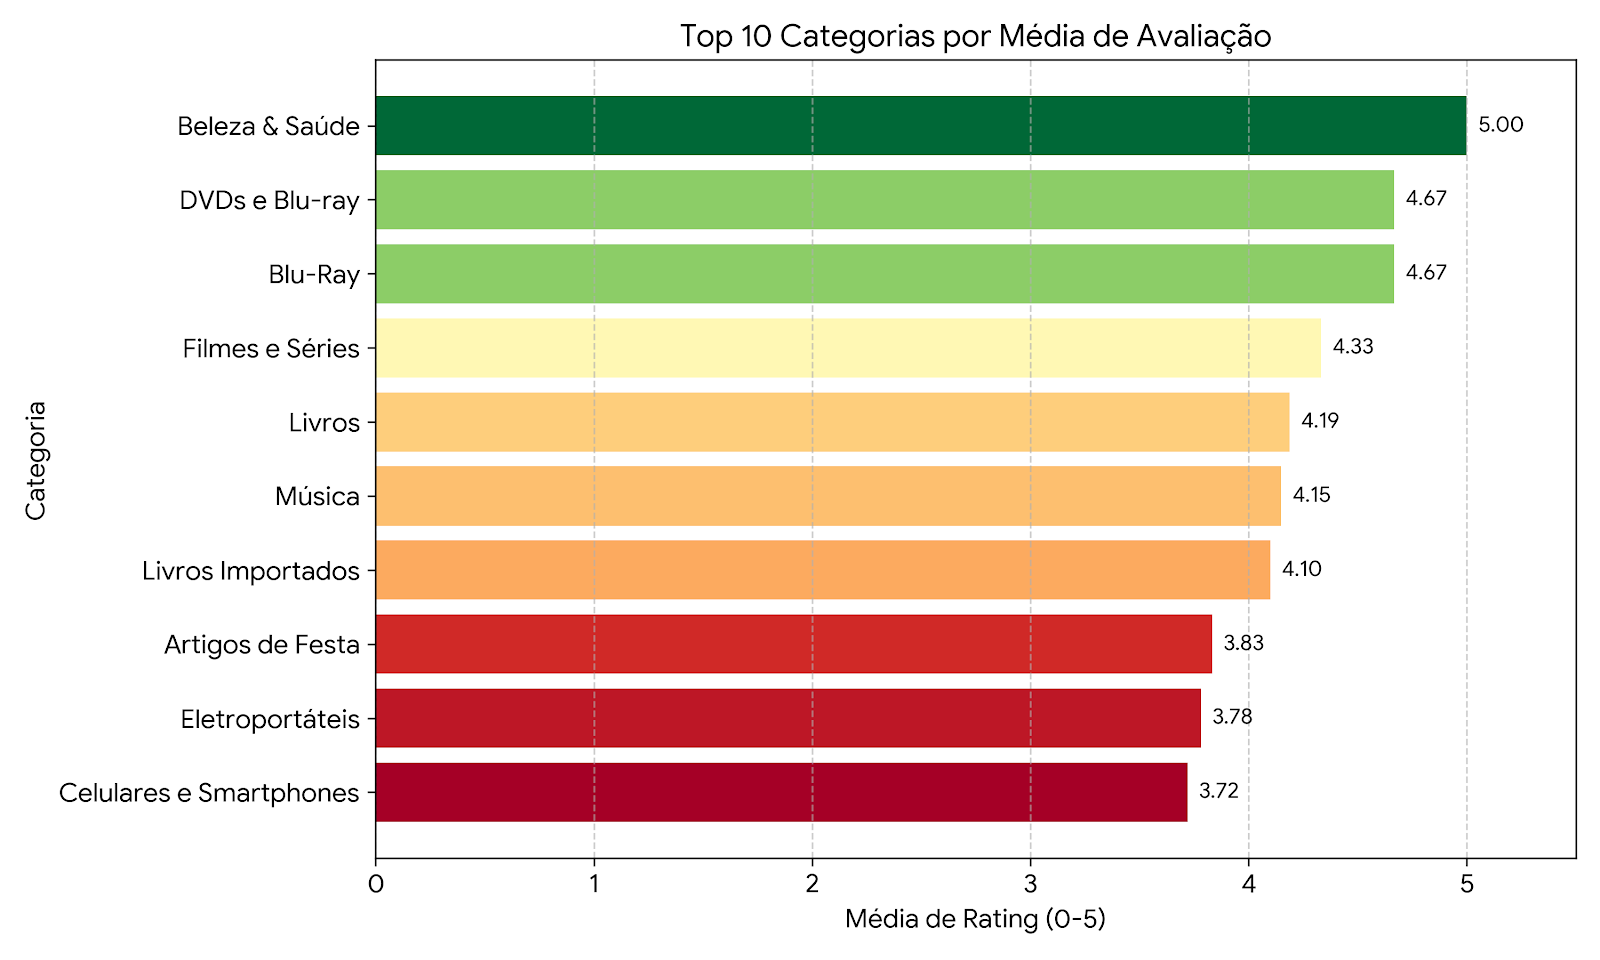
\includegraphics[width=\columnwidth]{figuras/tp_ranking_por_categoria.png}
    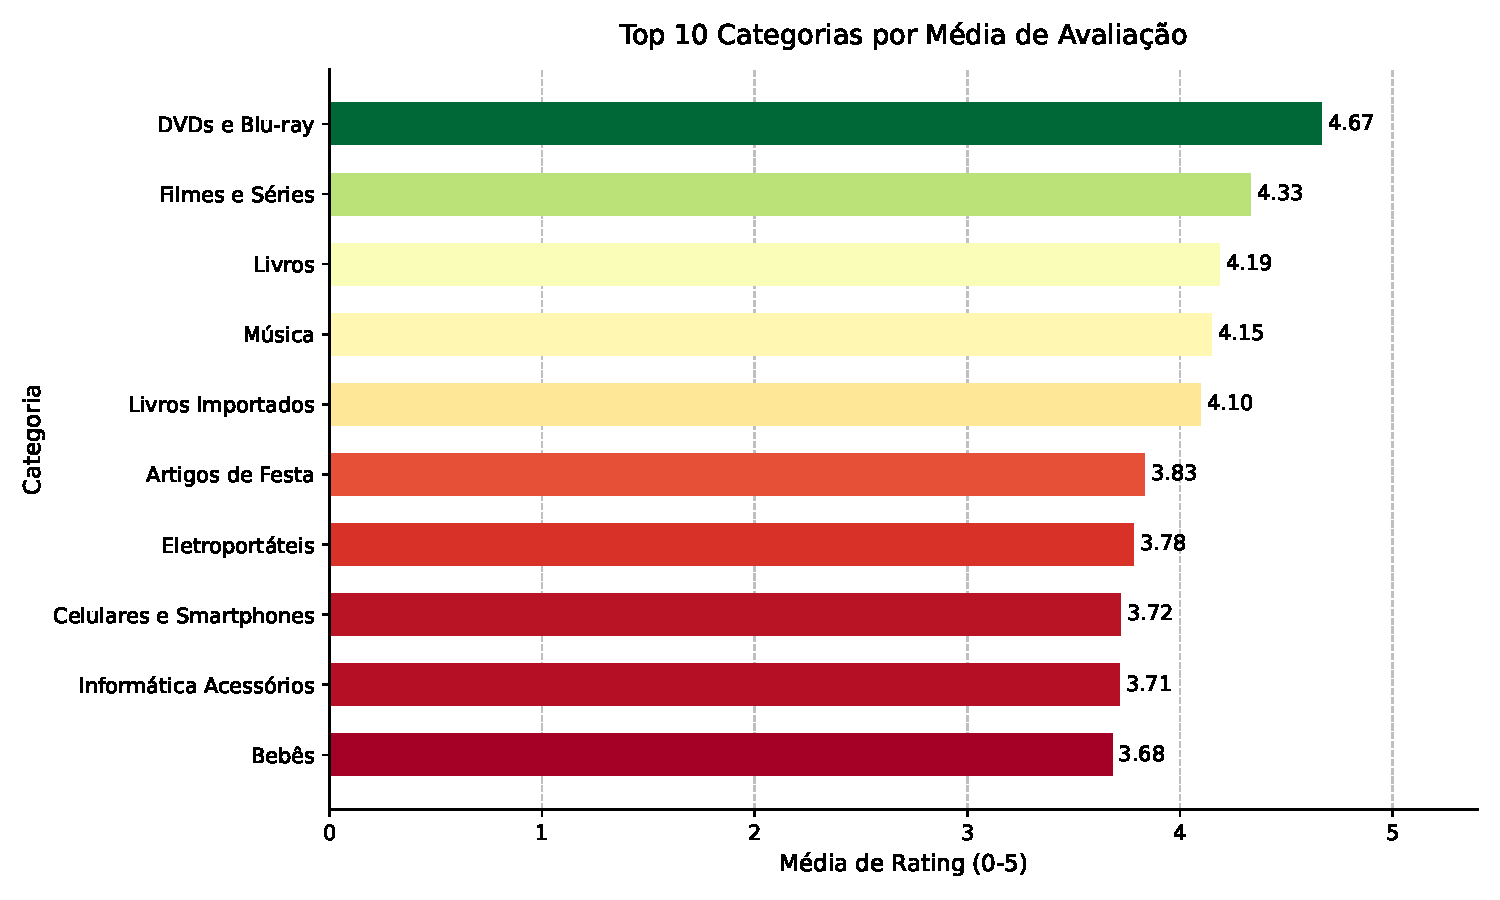
\includegraphics[width=\columnwidth]{figuras/grafico_top_rating_categorias.pdf}
    \caption{Média de avaliação por categoria de produto. Categorias de entretenimento e mídia física (DVDs, Blu-ray, Livros) concentram as maiores médias, enquanto Celulares e Smartphones e Eletroportáteis, categorias com maior volume de avaliações, apresentam as menores médias, sugerindo maior incidência de experiências negativas nesses segmentos.}
    \label{fig:ranking_categoria}
\end{figure}

\begin{figure}[htbp]
    \centering
    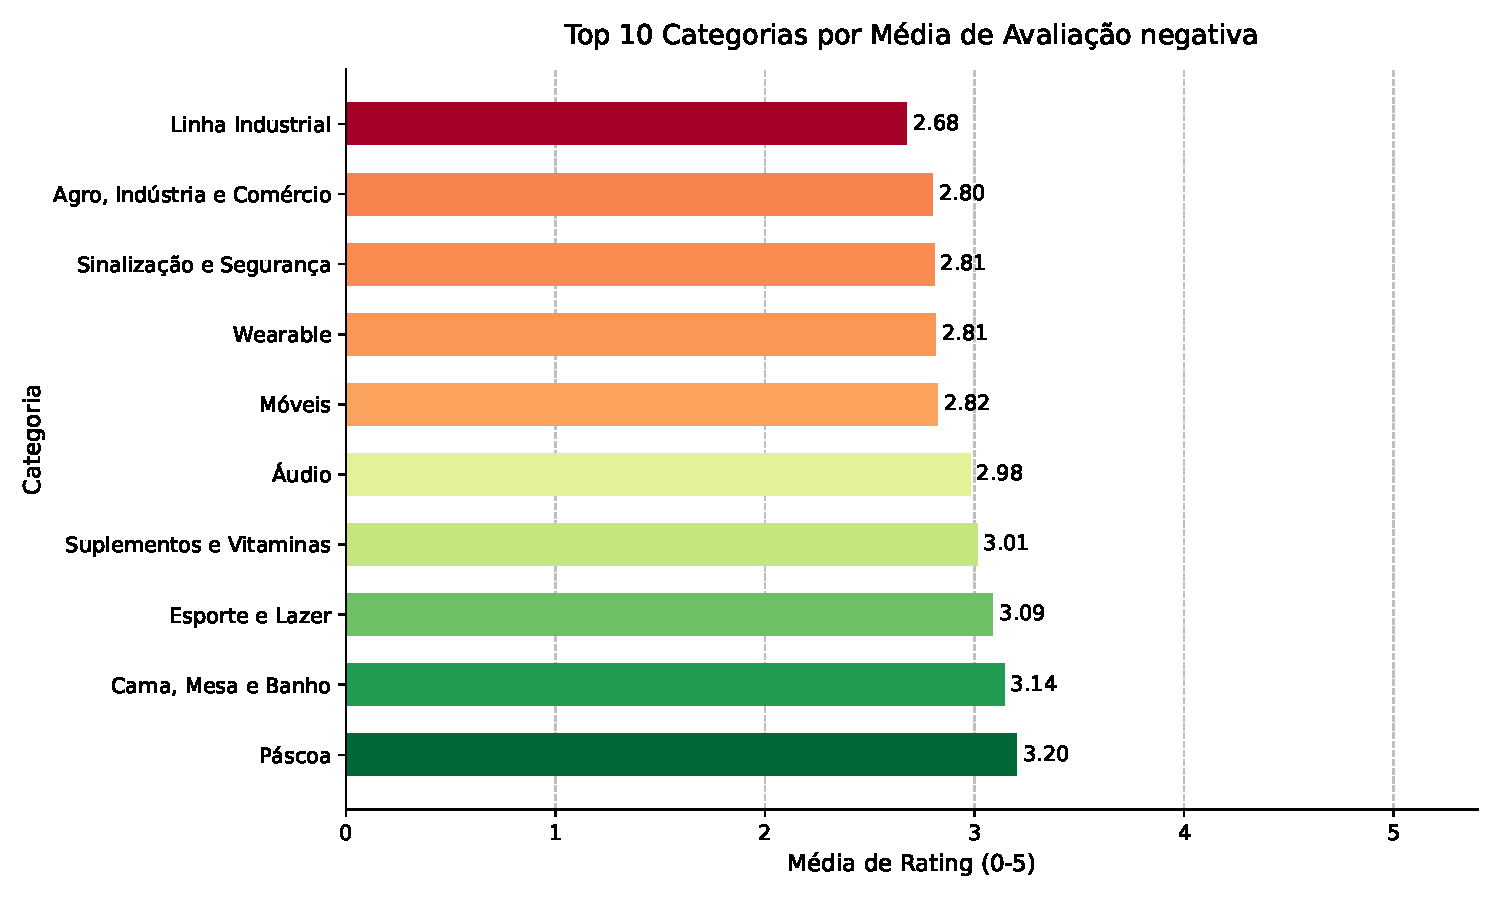
\includegraphics[width=\columnwidth]{figuras/grafico_bottom_rating_categorias.pdf}
    \caption{Top 10 categorias com menor média de avaliação no corpus. Linha Industrial, Agro, Indústria e Comércio e Sinalização e Segurança concentram as piores médias, todas abaixo de 3,0, sugerindo que categorias de nicho e baixo volume podem apresentar maior proporção de avaliações negativas.}
    \label{fig:ranking_negativo_categoria}
\end{figure}

\subsection{Visão Geral dos Pipelines}
\label{subsec:pipelines}

O projeto é composto por dois pipelines principais, apresentados nas Figuras~\ref{fig:pipeline_classification} e \ref{fig:pipeline_recommendation}. O primeiro abrange desde a ingestão dos dados brutos até a seleção do modelo campeão de classificação de sentimento. O segundo consome as saídas do modelo campeão para construir e avaliar o motor de recomendação orientado por sentimento.


\begin{figure}[htbp]
  \centering
  \small
  \sffamily
  \setlength{\extrarowheight}{3pt}

  \definecolor{colorIngestao}{HTML}{1A4D3E}
  \definecolor{colorRepres}{HTML}{3B2F85}
  \definecolor{colorClassif}{HTML}{5C2A18}
  \definecolor{colorAvaliacao}{HTML}{0F4C81}
  \definecolor{colorSaida}{HTML}{1E5618}
  \definecolor{colorSubtexto}{HTML}{E5E7EB}

  \begin{tabular}{c}

    \begin{tabular}{|p{5.5cm}|}
      \hline
      \rowcolor{colorIngestao}
      \centering \textcolor{white}{\textbf{Corpus B2W-Reviews01}} \tabularnewline
      \rowcolor{colorIngestao}
      \centering \textcolor{colorSubtexto}{\footnotesize Avaliações brutas em português brasileiro} \tabularnewline
      \hline
    \end{tabular} \\
    $\downarrow$ \\

    \begin{tabular}{|p{5.5cm}|}
      \hline
      \rowcolor{colorIngestao}
      \centering \textcolor{white}{\textbf{Mapeamento de Polaridade}} \tabularnewline
      \rowcolor{colorIngestao}
      \centering \textcolor{colorSubtexto}{\footnotesize Notas 1--2: negativo $\cdot$ Notas 4--5: positivo $\cdot$ Nota 3: descartada} \tabularnewline
      \hline
    \end{tabular} \\
    $\downarrow$ \\

    \begin{tabular}{|p{5.5cm}|}
      \hline
      \rowcolor{colorIngestao}
      \centering \textcolor{white}{\textbf{Análise Exploratória (EDA)}} \tabularnewline
      \rowcolor{colorIngestao}
      \centering \textcolor{colorSubtexto}{\footnotesize Distribuição de classes, dados faltantes e estatísticas} \tabularnewline
      \hline
    \end{tabular} \\
    $\downarrow$ \\

    \begin{tabular}{|p{5.5cm}|}
      \hline
      \rowcolor{colorIngestao}
      \centering \textcolor{white}{\textbf{Balanceamento de Classes}} \tabularnewline
      \rowcolor{colorIngestao}
      \centering \textcolor{colorSubtexto}{\footnotesize Pesos por classe no treinamento} \tabularnewline
      \hline
    \end{tabular} \\
    $\downarrow$ \\

    \begin{tabular}{|p{5.5cm}|}
      \hline
      \rowcolor{colorIngestao}
      \centering \textcolor{white}{\textbf{Divisão Estratificada}} \tabularnewline
      \rowcolor{colorIngestao}
      \centering \textcolor{colorSubtexto}{\footnotesize Treino 70\% $\cdot$ Validação 15\% $\cdot$ Teste 15\%} \tabularnewline
      \hline
    \end{tabular} \\
    $\downarrow$ \\

    \begin{tabular}{|p{5.5cm}|}
      \hline
      \rowcolor{colorIngestao}
      \centering \textcolor{white}{\textbf{Pré-processamento Textual}} \tabularnewline
      \rowcolor{colorIngestao}
      \centering \textcolor{colorSubtexto}{\footnotesize Normalização $\cdot$ tokenização $\cdot$ lematização (TF-IDF)} \tabularnewline
      \hline
    \end{tabular} \\
    $\downarrow$ \\

    \begin{tabular}{|p{5.5cm}|}
      \hline
      \rowcolor{colorRepres}
      \centering \textcolor{white}{\textbf{Representação da Informação}} \tabularnewline
      \rowcolor{colorRepres}
      \centering \textcolor{white}{\footnotesize $\bullet$ TF-IDF (uni e bigramas)} \tabularnewline
      \rowcolor{colorRepres}
      \centering \textcolor{white}{\footnotesize $\bullet$ BERTimbau \texttt{[CLS]} (pesos congelados)} \tabularnewline
      \rowcolor{colorRepres}
      \centering \textcolor{white}{\footnotesize $\bullet$ BERTimbau fine-tuning} \tabularnewline
      \hline
    \end{tabular} \\
    $\downarrow$ \\

    \begin{tabular}{|p{5.5cm}|}
      \hline
      \rowcolor{colorClassif}
      \centering \textcolor{white}{\textbf{Treinamento dos Modelos}} \tabularnewline
      \rowcolor{colorClassif}
      \centering \textcolor{white}{\footnotesize $\bullet$ TF-IDF + Regressão Logística} \tabularnewline
      \rowcolor{colorClassif}
      \centering \textcolor{white}{\footnotesize $\bullet$ BERTimbau + Regressão Logística} \tabularnewline
      \rowcolor{colorClassif}
      \centering \textcolor{white}{\footnotesize $\bullet$ BERTimbau fine-tuning + MLP} \tabularnewline
      \hline
    \end{tabular} \\
    $\downarrow$ \\

    \begin{tabular}{|p{5.5cm}|}
      \hline
      \rowcolor{colorAvaliacao}
      \centering \textcolor{white}{\textbf{Validação Cruzada Estratificada}} \tabularnewline
      \rowcolor{colorAvaliacao}
      \centering \textcolor{colorSubtexto}{\footnotesize TF-IDF: $k=5$ com Grid Search $\cdot$ BERTimbau: $k=3$} \tabularnewline
      \hline
    \end{tabular} \\
    $\downarrow$ \\

    \begin{tabular}{|p{5.5cm}|}
      \hline
      \rowcolor{colorAvaliacao}
      \centering \textcolor{white}{\textbf{Avaliação Quantitativa}} \tabularnewline
      \rowcolor{colorAvaliacao}
      \centering \textcolor{white}{\footnotesize $\bullet$ F1-macro $\quad$ $\bullet$ AUC-ROC} \tabularnewline
      \rowcolor{colorAvaliacao}
      \centering \textcolor{white}{\footnotesize $\bullet$ Precisão $\quad$ $\bullet$ Revocação $\quad$ $\bullet$ Matriz de Confusão} \tabularnewline
      \hline
    \end{tabular} \\
    $\downarrow$ \\

    \begin{tabular}{|p{5.5cm}|}
      \hline
      \rowcolor{colorAvaliacao}
      \centering \textcolor{white}{\textbf{Avaliação Qualitativa}} \tabularnewline
      \rowcolor{colorAvaliacao}
      \centering \textcolor{colorSubtexto}{\footnotesize Inspeção manual (90 instâncias) $\cdot$ Kappa de Cohen} \tabularnewline
      \hline
    \end{tabular} \\
    $\downarrow$ \\

    \begin{tabular}{|p{5.5cm}|}
      \hline
      \rowcolor{colorSaida}
      \centering \textcolor{white}{\textbf{Seleção do Modelo Campeão}} \tabularnewline
      \rowcolor{colorSaida}
      \centering \textcolor{colorSubtexto}{\footnotesize Melhor F1-macro no conjunto de teste} \tabularnewline
      \hline
    \end{tabular} \\
    \bigskip \\

    \begin{tabular}{lll}
      \fcolorbox{black}{colorIngestao}{\rule{0pt}{4pt}\rule{4pt}{0pt}} \footnotesize Ingestão e Preparação &
      \fcolorbox{black}{colorRepres}{\rule{0pt}{4pt}\rule{4pt}{0pt}} \footnotesize Representação &
      \fcolorbox{black}{colorClassif}{\rule{0pt}{4pt}\rule{4pt}{0pt}} \footnotesize Modelagem \\
      \fcolorbox{black}{colorAvaliacao}{\rule{0pt}{4pt}\rule{4pt}{0pt}} \footnotesize Avaliação &
      \fcolorbox{black}{colorSaida}{\rule{0pt}{4pt}\rule{4pt}{0pt}} \footnotesize Saída &
    \end{tabular}

  \end{tabular}
  \caption{Pipeline de classificação de sentimento sobre o corpus B2W-Reviews01, desde a ingestão dos dados brutos até a seleção do modelo campeão.}
  \label{fig:pipeline_classification}
\end{figure}

\begin{figure}[htbp]
  \centering
  \small
  \sffamily
  \setlength{\extrarowheight}{3pt}

  \definecolor{colorIngestao}{HTML}{1A4D3E}
  \definecolor{colorRepres}{HTML}{3B2F85}
  \definecolor{colorClassif}{HTML}{5C2A18}
  \definecolor{colorAvaliacao}{HTML}{0F4C81}
  \definecolor{colorSaida}{HTML}{1E5618}
  \definecolor{colorSubtexto}{HTML}{E5E7EB}

  \begin{tabular}{c}

    \begin{tabular}{|p{6.0cm}|}
      \hline
      \rowcolor{colorIngestao}
      \centering \textcolor{white}{\textbf{Classificação do Corpus Completo}} \tabularnewline
      \rowcolor{colorIngestao}
      \centering \textcolor{colorSubtexto}{\footnotesize Inferência com modelo campeão (Pipeline 1)} \tabularnewline
      \hline
    \end{tabular} \\
    $\downarrow$ \\

    \begin{tabular}{|p{6.0cm}|}
      \hline
      \rowcolor{colorIngestao}
      \centering \textcolor{white}{\textbf{Score de Sentimento por Produto}} \tabularnewline
      \rowcolor{colorIngestao}
      \centering \textcolor{colorSubtexto}{\footnotesize Proporção de avaliações positivas $\cdot$ mínimo de 5 avaliações} \tabularnewline
      \hline
    \end{tabular} \\
    $\downarrow$ \\

    \begin{tabular}{|p{6.0cm}|}
      \hline
      \rowcolor{colorRepres}
      \centering \textcolor{white}{\textbf{Vetorização dos Títulos}} \tabularnewline
      \rowcolor{colorRepres}
      \centering \textcolor{white}{\footnotesize Serafim PT* (335M) $\cdot$ mean pooling $\cdot$ 1024 dimensões} \tabularnewline
      \hline
    \end{tabular} \\
    $\downarrow$ \\

    \begin{tabular}{|p{6.0cm}|}
      \hline
      \rowcolor{colorClassif}
      \centering \textcolor{white}{\textbf{Indexação em Banco Vetorial}} \tabularnewline
      \rowcolor{colorClassif}
      \centering \textcolor{colorSubtexto}{\footnotesize FAISS $\cdot$ ChromaDB $\cdot$ Qdrant (a definir)} \tabularnewline
      \hline
    \end{tabular} \\
    $\downarrow$ \\

    \begin{tabular}{|p{6.0cm}|}
      \hline
      \rowcolor{colorClassif}
      \centering \textcolor{white}{\textbf{Busca e Recuperação (ANN)}} \tabularnewline
      \rowcolor{colorClassif}
      \centering \textcolor{colorSubtexto}{\footnotesize Top-K candidatos via similaridade de cosseno} \tabularnewline
      \hline
    \end{tabular} \\
    $\downarrow$ \\

    \begin{tabular}{|p{6.0cm}|}
      \hline
      \rowcolor{colorClassif}
      \centering \textcolor{white}{\textbf{Re-ranqueamento por Sentimento}} \tabularnewline
      \rowcolor{colorClassif}
      \centering \textcolor{colorSubtexto}{\footnotesize Combinação ponderada de similaridade e score de sentimento} \tabularnewline
      \hline
    \end{tabular} \\
    $\downarrow$ \\

    \begin{tabular}{|p{6.0cm}|}
      \hline
      \rowcolor{colorAvaliacao}
      \centering \textcolor{white}{\textbf{Avaliação Quantitativa}} \tabularnewline
      \rowcolor{colorAvaliacao}
      \centering \textcolor{white}{\footnotesize $\bullet$ NDCG@k $\quad$ $\bullet$ Precision@k} \tabularnewline
      \rowcolor{colorAvaliacao}
      \centering \textcolor{white}{\footnotesize $\bullet$ Recall@k $\quad$} \tabularnewline
      \hline
    \end{tabular} \\
    $\downarrow$ \\

    \begin{tabular}{|p{6.0cm}|}
      \hline
      \rowcolor{colorAvaliacao}
      \centering \textcolor{white}{\textbf{Avaliação Qualitativa}} \tabularnewline
      \rowcolor{colorAvaliacao}
      \centering \textcolor{colorSubtexto}{\footnotesize 20 pares consulta-lista $\cdot$ Kappa de Cohen} \tabularnewline
      \hline
    \end{tabular} \\
    $\downarrow$ \\

    \begin{tabular}{|p{6.0cm}|}
      \hline
      \rowcolor{colorSaida}
      \centering \textcolor{white}{\textbf{Lista Final de Recomendações}} \tabularnewline
      \rowcolor{colorSaida}
      \centering \textcolor{colorSubtexto}{\footnotesize Top-k produtos ordenados por relevância semântica e sentimento} \tabularnewline
      \hline
    \end{tabular} \\
    \bigskip \\

    \begin{tabular}{lll}
      \fcolorbox{black}{colorIngestao}{\rule{0pt}{4pt}\rule{4pt}{0pt}} \footnotesize Processamento Inicial &
      \fcolorbox{black}{colorRepres}{\rule{0pt}{4pt}\rule{4pt}{0pt}} \footnotesize Representação &
      \fcolorbox{black}{colorClassif}{\rule{0pt}{4pt}\rule{4pt}{0pt}} \footnotesize Recuperação / Ranking \\
      \fcolorbox{black}{colorAvaliacao}{\rule{0pt}{4pt}\rule{4pt}{0pt}} \footnotesize Avaliação &
      \fcolorbox{black}{colorSaida}{\rule{0pt}{4pt}\rule{4pt}{0pt}} \footnotesize Saída &
    \end{tabular}

  \end{tabular}
  \caption{Pipeline de recomendação orientada por sentimento, consumindo as saídas do modelo campeão para construir e avaliar o motor de recuperação e re-ranqueamento.}
  \label{fig:pipeline_recommendation}
\end{figure}


% \begin{figure}[htbp]
%   \centering
%   \fbox{\parbox{0.9\linewidth}{\centering
%     \textit{[Ver Figura separada: Pipeline de Recomendação]}\\
%     {\footnotesize Diagrama gerado como artefato complementar}
%   }}
%   \caption{Pipeline de Recomendação Orientada por Sentimento (Pipeline 2).}
%   \label{fig:pipeline_recommendation}
% \end{figure}

\subsection{Pipeline 1 -- Classificação de Sentimento}
\label{subsec:pipeline1}

\subsubsection{Divisão dos Dados}
\label{subsubsec:split}

Os dados serão divididos em três partições estratificadas por classe de sentimento:

\begin{itemize}[noitemsep]
  \item \textbf{Treino}: 70\% dos dados.
  \item \textbf{Validação}: 15\% dos dados (ajuste de hiperparâmetros).
  \item \textbf{Teste}: 15\% dos dados (avaliação final, utilizado apenas uma vez).
\end{itemize}

A estratificação garante que a proporção de classes positivas e negativas seja preservada em cada partição.

\subsubsection{Pré-processamento Textual}
\label{subsubsec:preprocessing}

A entrada dos modelos será o campo \texttt{review\_text} concatenado ao campo \texttt{review\_title}. O pré-processamento segue as etapas descritas a seguir, calibradas conforme o tipo de representação utilizada.

\paragraph{Normalização textual (aplicada a ambas as representações)}
\begin{enumerate}[noitemsep]
  \item Conversão para minúsculas (\textit{lowercasing}).
  \item Remoção de HTML tags, URLs e caracteres especiais não-alfanuméricos.
  \item Normalização de acentuação e caracteres Unicode (NFD/NFC).
  \item Remoção de espaços duplicados e linhas vazias.
\end{enumerate}

\paragraph{Pré-processamento adicional para TF-IDF (representação esparsa):}
\begin{enumerate}[noitemsep]
  \item Tokenização por espaço e pontuação.
  \item Remoção de \textit{stopwords} em português (lista NLTK).
  \item Lematização com spaCy.
  \item Construção do vocabulário e aplicação do TF-IDF com n-gramas de 1 a 2 (\textit{unigrams} e \textit{bigrams}). A inclusão de bigramas permite capturar associações locais entre termos adjacentes relevantes para o domínio, como ``não recebi'', ``boa qualidade'' e ``prazo entrega'', que perdem seu sentido quando analisadas como tokens isolados.
\end{enumerate}

\paragraph{Pré-processamento para Embeddings (representação densa)}
O BERTimbau utiliza seu próprio tokenizador \textit{WordPiece}, que lida internamente com vocabulário, subpalavras e tokens especiais ([CLS], [SEP]). Para este modelo, aplica-se apenas a normalização textual básica, preservando a estrutura morfológica necessária para o modelo contextual.

\subsubsection{Representação da Informação}
\label{subsubsec:representation}

\paragraph{Estratégia 1 -- TF-IDF (linha de base esparsa):}
Será construída uma matriz TF-IDF com os termos mais frequentes, aplicando suavização logarítmica no cálculo do IDF para lidar com termos raros. A ponderação TF-IDF é definida pela equação:

\begin{equation}
  \text{TF-IDF}(t,d,D) = \text{TF}(t,d) \times \log\!\left(\frac{N}{n_t}\right)
  \label{eq:tfidf}
\end{equation}

onde $N$ é o total de documentos e $n_t$ é o número de documentos que contêm o termo $t$.

\paragraph{Estratégia 2 -- Embeddings com BERTimbau:}
Utilizaremos o BERTimbau Base \cite{souza2020bertimbau} via Hugging Face. Serão investigadas duas configurações: (a) \textit{feature extraction}, em que os pesos do BERT são congelados e o vetor do token [CLS] é usado como representação de entrada para um classificador externo; e (b) \textit{fine-tuning} completo, em que uma camada linear é adicionada ao [CLS] e toda a rede é ajustada na tarefa de classificação binária.

\subsubsection{Modelos de Classificação}
\label{subsubsec:classifiers}

Para cada representação, serão treinados os seguintes modelos:

\begin{itemize}[noitemsep]
  \item \textbf{TF-IDF + RL}: linha de base com representação esparsa e classificador linear.
  \item \textbf{BERTimbau + RL}: embedding contextual \texttt{[CLS]} com pesos congelados e classificador linear.
  \item \textbf{BERTimbau fine-tuning + MLP}: encoder ajustado à tarefa com classificador não-linear treinado ponta-a-ponta.
\end{itemize}

\subsubsection{Validação e Seleção do Modelo}
\label{subsubsec:validation}
Todos os modelos serão avaliados com validação cruzada estratificada sobre o conjunto de treino e validação, garantindo comparabilidade entre as configurações. Para os modelos baseados em TF-IDF, serão utilizados $k=5$ \textit{folds} com otimização de hiperparâmetros via \textit{Grid Search}. Para os modelos BERTimbau, dado o maior custo computacional, serão utilizados $k=3$ \textit{folds}. Em ambos os casos, o modelo com melhor F1-macro médio entre os \textit{folds} será selecionado para avaliação final no conjunto de teste.

\subsubsection{Métricas de Avaliação -- Classificação}
\label{subsubsec:metrics_classification}

As métricas utilizadas para avaliar os modelos de classificação de sentimento são:

\begin{itemize}[noitemsep]
  \item \textbf{Precisão (P)}: proporção de predições positivas corretas.
  \item \textbf{Revocação (R)}: proporção de positivos verdadeiros recuperados.
  \item \textbf{F1-score macro}: média harmônica de P e R, calculada por classe e depois com média macro (sem ponderação por frequência de classe), definida como:
    \begin{equation}
      F_1 = \frac{2 \cdot P \cdot R}{P + R}
      \label{eq:f1}
    \end{equation}
  \item \textbf{AUC-ROC}: área sob a curva ROC, medida de discriminação do modelo independente do limiar de decisão.
  \item \textbf{Matriz de confusão}: análise qualitativa dos tipos de erro (falsos positivos e falsos negativos).
\end{itemize}

\subsubsection{Avaliação Qualitativa}
\label{subsubsec:qual_classification}

Uma amostra aleatória estratificada de 90 instâncias do conjunto de teste será avaliada manualmente por pelo menos dois integrantes do grupo, de forma independente, quanto à polaridade real do texto. Os rótulos humanos serão comparados aos rótulos automáticos do modelo campeão. Será calculado o coeficiente de concordância Kappa de Cohen entre os avaliadores humanos.

\subsection{Pipeline 2 -- Recomendação Orientada por Sentimento}
\label{subsec:pipeline2}

\subsubsection{Score de Sentimento por Produto}
\label{subsubsec:sentiment_score}

O modelo campeão da etapa de classificação será aplicado a todas as avaliações do corpus para classificá-las como positivas ou negativas. Para cada produto único (identificado pelo \texttt{product\_id}), será calculado um \textit{score} de relevância $S(p)$ definido como:

\begin{equation}
  S(p) = \frac{|\{\text{avaliações positivas de } p\}|}{|\{\text{todas as avaliações de } p\}|}
  \label{eq:score}
\end{equation}

Apenas produtos com ao menos $n_{\min}=5$ avaliações serão incluídos no índice de recomendação, de modo a garantir confiabilidade estatística do score.

\subsubsection{Vetorização dos Títulos de Produtos}
\label{subsubsec:vectorization}
Os títulos de produto (\texttt{product\_name}) serão vetorizados utilizando o Serafim PT* \cite{gomes2024serafim}, uma família de sentence encoders abertos para o português com desempenho competitivo em tarefas de similaridade semântica e recuperação de informação. Será utilizada a variante \texttt{serafim-335m-portuguese-pt-sentence-encoder}, que produz vetores densos de 1024 dimensões via \textit{mean pooling}, adequados para indexação e busca por similaridade de cosseno no banco vetorial.

\subsubsection{Banco Vetorial e Recuperação}
\label{subsubsec:vectordb}

Os vetores de título serão indexados em um banco vetorial \textit{open-source}, com candidatos como FAISS, ChromaDB e Qdrant, cuja escolha será definida na etapa de implementação. A busca por similaridade será realizada por \textit{Approximate Nearest Neighbors} (ANN) com cosseno como métrica de distância:

\begin{equation}
  \text{sim}(\vec{u}, \vec{v}) = \frac{\vec{u} \cdot \vec{v}}{|\vec{u}|\, |\vec{v}|}
  \label{eq:cosine}
\end{equation}

Dado um produto de consulta $q$, o sistema recupera os $K$ títulos mais similares do índice, cujo valor será definido empiricamente durante a validação do módulo de recomendação.

\subsubsection{Re-ranqueamento por Sentimento}
\label{subsubsec:reranking}

Os $K$ candidatos recuperados são re-ranqueados pela seguinte pontuação combinada:

\begin{equation}
  \text{Score}_{\text{final}}(p) = \alpha \cdot \text{sim}(q, p) + (1 - \alpha) \cdot S(p)
  \label{eq:reranking}
\end{equation}

onde $\alpha \in [0, 1]$ é um hiperparâmetro que controla o trade-off entre similaridade semântica e positividade percebida do produto. Os produtos são ordenados de forma decrescente por $\text{Score}_{\text{final}}$ e os $k$ primeiros são retornados como recomendações.

\subsubsection{Métricas de Avaliação -- Recomendação}
\label{subsubsec:metrics_recomendation}

Para avaliar o módulo de recomendação, serão utilizadas as seguintes métricas baseadas em ranking:

\begin{itemize}[noitemsep]
  \item \textbf{Precision@k}: proporção de itens relevantes nos $k$ primeiros retornados.
  \item \textbf{Recall@k}: proporção de itens relevantes recuperados entre todos os relevantes.
  \item \textbf{NDCG@k} (\textit{Normalized Discounted Cumulative Gain}): penaliza a posição dos itens relevantes na lista, favorecendo listas em que os melhores itens aparecem primeiro:
    \begin{equation}
      \text{NDCG}@k = \frac{\text{DCG}@k}{\text{IDCG}@k}, \quad \text{DCG}@k = \sum_{i=1}^{k} \frac{2^{r_i}-1}{\log_2(i+1)}
      \label{eq:ndcg}
    \end{equation}
    onde $r_i$ é a relevância do item na posição $i$.
\end{itemize}

Para a avaliação do re-ranqueamento, produtos com $S(p) > 0.7$ serão considerados ``altamente relevantes'' e produtos com $S(p) < 0.3$ como ``pouco relevantes'', criando um conjunto de referência para o cálculo das métricas acima.

\subsubsection{Avaliação Qualitativa -- Recomendação}
\label{subsubsec:qual_recommendation}

Cada integrante do grupo avaliará de forma independente uma amostra de 20 pares consulta-lista-recomendada, julgando se as recomendações são: (a) semanticamente relevantes para o produto de consulta; (b) de alta qualidade percebida (score de sentimento elevado); e (c) diversas o suficiente para agregar valor. A concordância entre avaliadores será novamente medida pelo Kappa de Cohen.

% =========================================================
\section{Considerações Finais}
\label{sec:conclusion}

Este relatório parcial apresenta a proposta do projeto para a disciplina de Processamento de Linguagem Natural. O projeto aborda o problema de recomendação de produtos em e-commerce em português brasileiro, propondo a integração de análise de sentimentos com recuperação semântica por similaridade vetorial de títulos de produtos.

A abordagem em duas etapas, classificação de sentimento seguida de recomendação re-ranqueada, parte de uma análise exploratória do corpus B2W-Reviews01 que já aponta desafios relevantes: ruído linguístico, desalinhamento entre texto e nota, e heterogeneidade de domínio entre categorias de produto. O uso do TF-IDF como linha de base, combinado com o BERTimbau em duas configurações distintas, permitirá avaliar a contribuição da representação contextual frente a abordagens esparsas em um domínio de texto coloquial e ruidoso. O módulo de recomendação, apoiado no Serafim PT* para vetorização de títulos e em um banco vetorial a ser definido, integra o sinal de sentimento ao processo de recuperação por meio de re-ranqueamento ponderado.

\paragraph{Próximos passos (a serem desenvolvidos até o Seminário 2):}
\begin{enumerate}[noitemsep]
  \item Conclusão da análise exploratória e consolidação das estatísticas do corpus.
  \item Implementação e treinamento dos três modelos de classificação definidos.
  \item Validação cruzada, otimização de hiperparâmetros e seleção do modelo campeão.
  \item Implementação do Pipeline 2: vetorização de títulos, indexação no banco vetorial e re-ranqueamento.
  \item Avaliação quantitativa do módulo de recomendação com as métricas de ranking definidas.
  \item Avaliação qualitativa independente por integrantes do grupo e cálculo do Kappa de Cohen.
\end{enumerate}

\bibliographystyle{IEEEtran}
\bibliography{references}

\end{document}